\section{Moments}
\label{sec:appendix:moments}

\subsection{Overview}
\subsubsection{Moments and initialization for addition}
The desired properties for initialization are according to Glorot et al. \cite{glorot-initialization}:
\begin{equation}
\begin{aligned}
E[z_{h_\ell}] &= 0 & E\left[\frac{\partial \mathcal{L}}{\partial z_{h_{\ell-1}}}\right] &= 0 \\
Var[z_{h_\ell}] &= Var\left[z_{h_{\ell-1}}\right] &
Var\left[\frac{\partial \mathcal{L}}{\partial z_{h_{\ell-1}}}\right] &= Var\left[\frac{\partial \mathcal{L}}{\partial z_{h_{\ell}}}\right]
\end{aligned}
\end{equation}

\subsubsection{Initialization for addition}

Glorot initialization can not be used for $\mathrm{NAC}_{+}$ as $W_{h_{\ell-1},h_{\ell}}$ is not sampled directly. Assuming that $\hat{W}_{h_\ell, h_{\ell-1}} \sim \mathrm{Uniform}[-r, r]$ and $\hat{M}_{h_\ell, h_{\ell-1}} \sim \mathrm{Uniform}[-r, r]$, then the variance can be derived (see proof in Appendix \ref{sec:appendix:moments:weight-matrix-construction}) to be:
\begin{equation}
Var[W_{h_{\ell-1},h_{\ell}}] = \frac{1}{2r} \left(1 - \frac{\tanh(r)}{r}\right) \left(r - \tanh\left(\frac{r}{2}\right)\right)
\end{equation}
One can then solve for $r$, given the desired variance ($Var[W_
{h_{\ell-1},h_{\ell}}] = \frac{2}{H_{\ell-1} + H_{\ell}}$) \cite{glorot-initialization}.

\subsubsection{Moments and initialization for multiplication}
Using second order multivariate Taylor approximation and some assumptions of uncorrelated stochastic variables, the expectation and variance of the $\mathrm{NAC}_{\bullet}$ layer can be estimated to:
\begin{equation}
\begin{aligned}
f(c_1, c_2) &= \left(1 + c_1 \frac{1}{2} Var[W_{h_\ell, h_{\ell-1}}] \log(|E[z_{h_{\ell-1}}]| + \epsilon)^2\right)^{c_2\ H_{\ell-1}} \\
E[z_{h_\ell}] &\approx f\left(1, 1\right) \\
Var[z_{h_\ell}] &\approx f\left(4, 1\right) - f\left(1, 2\right) \\
E\left[\frac{\partial \mathcal{L}}{\partial z_{h_{\ell-1}}}\right] &= 0 \\
Var\left[\frac{\partial \mathcal{L}}{\partial z_{h_{\ell-1}}}\right] &\approx Var\left[\frac{\partial \mathcal{L}}{\partial z_{h_{\ell}}}\right] H_{\ell}\ f\left(4, 1\right)\ Var[W_{h_{\ell}, h_{\ell-1}}] \\
&\cdot \left(\frac{1}{\left(|E[z_{h_{\ell-1}}]| + \epsilon\right)^2} + \frac{3}{\left(|E[z_{h_{\ell-1}}]| + \epsilon\right)^4} Var[z_{h_{\ell-1}}]\right)
\end{aligned}
\end{equation}

This is problematic because $E[z_{h_\ell}] \ge 1$, and the variance explodes for $E[z_{h_{\ell-1}}] = 0$. $E[z_{h_{\ell-1}}] = 0$ is normally a desired property \cite{glorot-initialization}. The variance explodes for $E[z_{h_{\ell-1}}] = 0$, and can thus not be initialized to anything meaningful.

For our proposed NMU, the expectation and variance can be derived (see proof in Appendix \ref{sec:appendix:moments:nmu}) using the same assumptions as before, although no Taylor approximation is required:
\begin{equation}
\begin{aligned}
E[z_{h_\ell}] &\approx \left(\frac{1}{2}\right)^{H_{\ell-1}} \\
E\left[\frac{\partial \mathcal{L}}{\partial z_{h_{\ell-1}}}\right] &\approx 0 \\
Var[z_{h_\ell}] &\approx \left(Var[W_{h_{\ell-1},h_\ell}] + \frac{1}{4}\right)^{H_{\ell-1}} \left(Var[z_{h_{\ell-1}}] + 1\right)^{H_{\ell-1}} - \left(\frac{1}{4}\right)^{H_{\ell-1}} \\
Var\left[\frac{\partial \mathcal{L}}{\partial z_{h_{\ell-1}}}\right] &\approx Var\left[\frac{\partial \mathcal{L}}{\partial z_{h_\ell}}\right] H_\ell \\
&\cdot \left(
\left(Var[W_{h_{\ell-1},h_\ell}] + \frac{1}{4}\right)^{H_{\ell-1}} \left(Var[z_{h_{\ell-1}}] + 1\right)^{H_{\ell-1} - 1}\right)
\end{aligned}
\end{equation}

These expectations are better behaved. It is properly unlikely to expect that the expectation can become zero, since the identity for multiplication is 1. However, for a large $H_{\ell-1}$ it will be near zero.

The variance is also better behaved, but does not provide a input-independent initialization strategy. We propose initializing with $Var[W_{h_{\ell-1},h_\ell}] = \frac{1}{4}$, as this is the solution to $Var[z_{h_\ell}] = Var[z_{h_{\ell-1}}]$ assuming $Var[z_{h_{\ell-1}}] = 1$ and a large $H_{\ell-1}$ (see proof in Appendix \ref{sec:appendix:moments:nmu:initialization}). However, feel free to compute more exact solutions.

\subsection{Expectation and variance for weight matrix construction in NAC layers}
\label{sec:appendix:moments:weight-matrix-construction}

The weight matrix construction in NAC, is defined in scalar notation as: 
\begin{equation}
W_{h_\ell, h_{\ell-1}} = \tanh(\hat{W}_{h_\ell, h_{\ell-1}}) \sigma(\hat{M}_{h_\ell, h_{\ell-1}})
\end{equation}

Simplifying the notation of this, and re-expressing it using stochastic variables with uniform distributions this can be written as:
\begin{equation}
\begin{aligned}
W &\sim \tanh(\hat{W}) \sigma(\hat{M}) \\
\hat{W} &\sim ~ U[-r, r] \\
\hat{M} &\sim ~ U[-r, r] 
\end{aligned}
\end{equation}

Since $\tanh({\hat{W}})$ is an odd-function and $E[\hat{W}] = 0$, deriving the expectation $E[W]$ is trivial.
\begin{equation}
\mathrm{E}[W] = \mathrm{E}[\tanh(\hat{W})]\mathrm{E}[\sigma(\hat{M})] = 0 \cdot \mathrm{E}[\sigma(\hat{M})] = 0
\end{equation}

The variance is more complicated, however as $\hat{W}$ and $\hat{M}$ are independent, it can be simplified to:
\begin{equation}
\mathrm{Var}[W] = \mathrm{E}[\tanh(\hat{W})^2] \mathrm{E}[\sigma(\hat{M})^2] - \mathrm{E}[\tanh(\hat{W})]^2 \mathrm{E}[\sigma(\hat{M})]^2 = \mathrm{E}[\tanh(\hat{W})^2] \mathrm{E}[\sigma(\hat{M})^2]
\end{equation}

These second moments can be analyzed independently. First for $\mathrm{E}[\tanh(\hat{W})^2]$:
\begin{equation}
\begin{aligned}
\mathrm{E}[\tanh(\hat{W})^2] &= \int_{-\infty}^{\infty} \tanh(x)^2 f_{U[-r, r]}(x)\ \mathrm{d}x \\
&= \frac{1}{2r} \int_{-r}^{r} \tanh(x)^2\ \mathrm{d}x \\
&= \frac{1}{2r} \cdot 2 \cdot (r - \tanh(r)) \\
&= 1 - \frac{\tanh(r)}{r}
\end{aligned}
\end{equation}

Then for $\mathrm{E}[\tanh(\hat{M})^2]$:
\begin{equation}
\begin{aligned}
\mathrm{E}[\sigma(\hat{M})^2] &= \int_{-\infty}^{\infty} \sigma(x)^2 f_{U[-r, r]}(x)\ \mathrm{d}x \\
&= \frac{1}{2r} \int_{-r}^{r} \sigma(x)^2\ \mathrm{d}x \\
&= \frac{1}{2r} \left(r - \tanh\left(\frac{r}{2}\right)\right)
\end{aligned}
\end{equation}

Finally this gives the variance:
\begin{equation}
\mathrm{Var}[W] = \frac{1}{2r} \left(1 - \frac{\tanh(r)}{r}\right) \left(r - \tanh\left(\frac{r}{2}\right)\right)
\end{equation}

\subsection{Expectation and variance of \texorpdfstring{$\mathrm{NAC}_{\bullet}$}{NAC-mul}}
\label{sec:appendix:moments:nac-mul}
\subsubsection{Forward pass}

\paragraph{Expectation} Assuming that each $z_{h_{\ell-1}}$ are uncorrelated the expectation can be simplified to:
\begin{equation}
\begin{aligned}
E[z_{h_\ell}] &= E\left[\exp\left(\sum_{h_{\ell-1}=1}^{H_{\ell-1}} W_{h_{\ell}, h_{\ell-1}} \log(|z_{h_{\ell-1}}| + \epsilon) \right)\right] \\
&= E\left[\prod_{h_{\ell-1}=1}^{H_{\ell-1}} \exp(W_{h_{\ell}, h_{\ell-1}} \log(|z_{h_{\ell-1}}| + \epsilon)) \right] \\
&\approx \prod_{h_{\ell-1}=1}^{H_{\ell-1}} E[\exp(W_{h_{\ell}, h_{\ell-1}} \log(|z_{h_{\ell-1}}| + \epsilon))] \\
&= E[\exp(W_{h_{\ell}, h_{\ell-1}} \log(|z_{h_{\ell-1}}| + \epsilon))]^{H_{\ell-1}} \\
&= E\left[(|z_{h_{\ell-1}}| + \epsilon)^{W_{h_{\ell}, h_{\ell-1}}}\right]^{H_{\ell-1}} \\
&= E\left[f(z_{h_{\ell-1}}, W_{h_{\ell}, h_{\ell-1}})\right]^{H_{\ell-1}}
\end{aligned}
\end{equation}

Here we define $g$ as a non-linear transformation function of two independent stochastic variables:
\begin{equation}
f(z_{h_{\ell-1}}, W_{h_{\ell}, h_{\ell-1}}) = (|z_{h_{\ell-1}}| + \epsilon)^{W_{h_{\ell}, h_{\ell-1}}}
\end{equation}

We then take the second order Taylor approximation of $g$, around $(E[z_{h_{\ell-1}}], E[W_{h_{\ell}, h_{\ell-1}}])$.
\begin{equation}
\begin{aligned}
&E[f(z_{h_{\ell-1}}, W_{h_{\ell}, h_{\ell-1}})] \approx
E\Bigg[\\
&g(E[z_{h_{\ell-1}}], E[W_{h_{\ell}, h_{\ell-1}}])\\
&+ \begin{bmatrix}
z_{h_{\ell-1}} - E[z_{h_{\ell-1}}] \\ W_{h_{\ell}, h_{\ell-1}} - E[W_{h_{\ell}, h_{\ell-1}}]
\end{bmatrix}^T \begin{bmatrix}
\frac{\partial g(z_{h_{\ell-1}}, W_{h_{\ell}, h_{\ell-1}})}{\partial z_{h_{\ell-1}}} \\
\frac{\partial g(z_{h_{\ell-1}}, W_{h_{\ell}, h_{\ell-1}})}{\partial W_{h_{\ell}, h_{\ell-1}}}
\end{bmatrix} \Bigg\rvert_{
\begin{cases}
z_{h_{\ell-1}} = E[z_{h_{\ell-1}}] \\
W_{h_{\ell}, h_{\ell-1}} = E[W_{h_{\ell}, h_{\ell-1}}]
\end{cases}
} \\
&+ \frac{1}{2} \begin{bmatrix}
z_{h_{\ell-1}} - E[z_{h_{\ell-1}}] \\ W_{h_{\ell}, h_{\ell-1}} - E[W_{h_{\ell}, h_{\ell-1}}]
\end{bmatrix}^T \\
&\bullet \begin{bmatrix}
\frac{\partial^2 g(z_{h_{\ell-1}}, W_{h_{\ell}, h_{\ell-1}})}{\partial^2 z_{h_{\ell-1}}} & \frac{\partial^2 g(z_{h_{\ell-1}}, W_{h_{\ell}, h_{\ell-1}})}{\partial z_{h_{\ell-1}} \partial W_{h_{\ell}, h_{\ell-1}}} \\
\frac{\partial^2 g(z_{h_{\ell-1}}, W_{h_{\ell}, h_{\ell-1}})}{\partial z_{h_{\ell-1}} \partial W_{h_{\ell}, h_{\ell-1}}} & \frac{\partial^2 g(z_{h_{\ell-1}}, W_{h_{\ell}, h_{\ell-1}})}{\partial^2 W_{h_{\ell}, h_{\ell-1}}}
\end{bmatrix} \Bigg\rvert_{
\begin{cases}
z_{h_{\ell-1}} = E[z_{h_{\ell-1}}] \\
W_{h_{\ell}, h_{\ell-1}} = E[W_{h_{\ell}, h_{\ell-1}}]
\end{cases}
} \\
&\bullet \begin{bmatrix}
z_{h_{\ell-1}} - E[z_{h_{\ell-1}}] \\ W_{h_{\ell}, h_{\ell-1}} - E[W_{h_{\ell}, h_{\ell-1}}]
\end{bmatrix}\Bigg]
\end{aligned}
\end{equation}

Because $E[z_{h_{\ell-1}} - E[z_{h_{\ell-1}}]] = 0$, $E[W_{h_{\ell}, h_{\ell-1}} - E[W_{h_{\ell}, h_{\ell-1}}]] = 0$, and $Cov[z_{h_{\ell-1}}, W_{h_{\ell}, h_{\ell-1}}] = 0$. This simplifies to:
\begin{equation}
\begin{aligned}
&E[g(z_{h_{\ell-1}}, W_{h_{\ell}, h_{\ell-1}})] \approx
g(E[z_{h_{\ell-1}}], E[W_{h_{\ell}, h_{\ell-1}}])\\
&+ \frac{1}{2} Var\begin{bmatrix}
z_{h_{\ell-1}} \\ W_{h_{\ell}, h_{\ell-1}}
\end{bmatrix}^T \begin{bmatrix}
\frac{\partial^2 g(z_{h_{\ell-1}}, W_{h_{\ell}, h_{\ell-1}})}{\partial^2 z_{h_{\ell-1}}} \\
\frac{\partial^2 g(z_{h_{\ell-1}}, W_{h_{\ell}, h_{\ell-1}})}{\partial^2 W_{h_{\ell}, h_{\ell-1}}}
\end{bmatrix} \Bigg\rvert_{
\begin{cases}
z_{h_{\ell-1}} = E[z_{h_{\ell-1}}] \\
W_{h_{\ell}, h_{\ell-1}} = E[W_{h_{\ell}, h_{\ell-1}}]
\end{cases}
}
\end{aligned}
\end{equation}

Inserting the derivatives and computing the inner products yields:
\begin{equation}
\begin{aligned}
&E[g(z_{h_{\ell-1}}, W_{h_{\ell}, h_{\ell-1}})] \approx
(|E[z_{h_{\ell-1}}]| + \epsilon)^{E[W_{h_{\ell}, h_{\ell-1}}]} \\
&+ \frac{1}{2} Var[z_{h_{\ell-1}}] (|E[z_{h_{\ell-1}}]| + \epsilon)^{E[W_{h_{\ell}, h_{\ell-1}}] - 2} E[W_{h_{\ell}, h_{\ell-1}}] (E[W_{h_{\ell}, h_{\ell-1}}] - 1) \\
&+ \frac{1}{2} Var[W_{h_{\ell}, h_{\ell-1}}] (|E[z_{h_{\ell-1}}]| + \epsilon)^{E[W_{h_{\ell}, h_{\ell-1}}]} \log(|E[z_{h_{\ell-1}}]| + \epsilon)^2 \\
&=1 + \frac{1}{2} Var[W_{h_{\ell}, h_{\ell-1}}] \log(|E[z_{h_{\ell-1}}]| + \epsilon)^2
\end{aligned}
\end{equation}

This gives the final expectation:
\begin{equation}
\begin{aligned}
E[z_{h_\ell}] &= E\left[g(z_{h_{\ell-1}}, W_{h_{\ell}, h_{\ell-1}})\right]^{H_{\ell-1}} \\
&\approx\left(1 + \frac{1}{2} Var[W_{h_{\ell}, h_{\ell-1}}] \log(|E[z_{h_{\ell-1}}]| + \epsilon)^2\right)^{H_{\ell-1}}
\end{aligned}
\end{equation}

As this expectation is of particular interest, we evaluate the error of the approximation, where $W_{h_{\ell}, h_{\ell-1}} \sim U[-r_w,r_w]$ and $z_{h_{\ell-1}} \sim U[0, r_z]$. These distributions are what is used in the  arithmetic dataset. The error is plotted in figure \ref{fig:nac-mul-expectation-estimate}.
\begin{figure}[h]
\centering
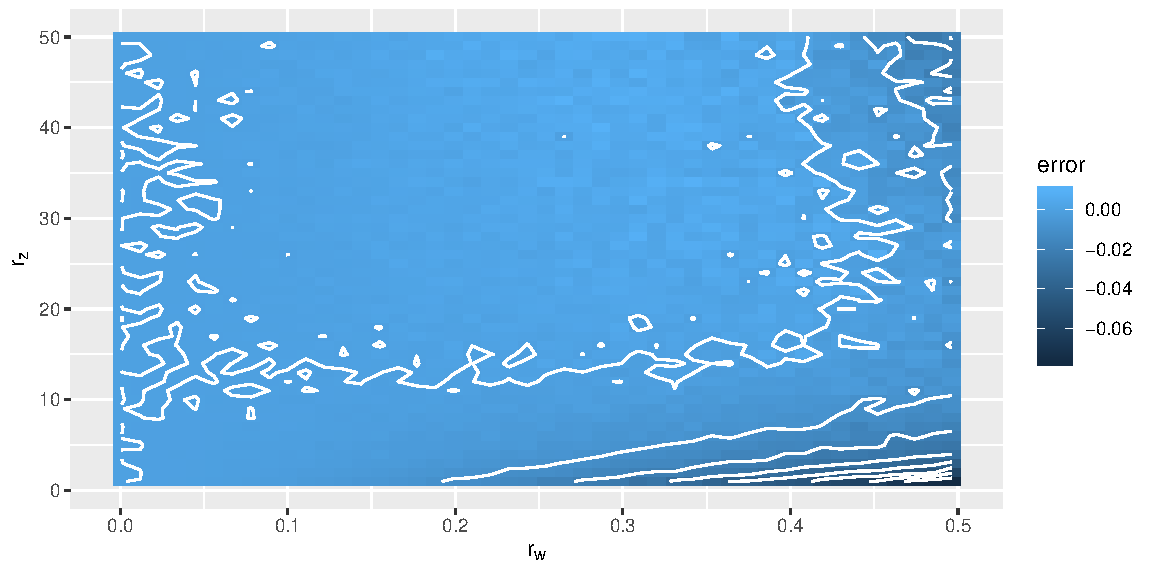
\includegraphics[width=\linewidth]{graphics/nac-mul-expectation-estimate.pdf}
\caption{Error between theoretical approximation and the numerical approximation estimated by random sampling of $100000$ observations at each combination of $r_z$ and $r_w$.}
\label{fig:nac-mul-expectation-estimate}
\end{figure}

\paragraph{Variance} The variance can be derived using the same assumptions for expectation, that all $z_{h_{\ell-1}}$ are uncorrelated.
\begin{equation}
\begin{aligned}
Var[z_{h_\ell}] &= E[z_{h_\ell}^2] - E[z_{h_\ell}]^2 \\
&= E\left[\prod_{h_{\ell-1}=1}^{H_{\ell-1}} (|z_{h_{\ell-1}}| + \epsilon)^{2 \cdot W_{h_{\ell}, h_{\ell-1}}} \right]
- E\left[\prod_{h_{\ell-1}=1}^{H_{\ell-1}} (|z_{h_{\ell-1}}| + \epsilon)^{W_{h_{\ell}, h_{\ell-1}}}\right]^2 \\
&= E\left[g(z_{h_{\ell-1}}, 2 \cdot W_{h_{\ell}, h_{\ell-1}}) \right]^{H_{\ell-1}}
- E\left[g(z_{h_{\ell-1}}, W_{h_{\ell}, h_{\ell-1}})\right]^{2\cdot H_{\ell-1}}
\end{aligned}
\end{equation}

We already have from the expectation result that:
\begin{equation}
E\left[g(z_{h_{\ell-1}}, W_{h_{\ell}, h_{\ell-1}})\right] \approx 1 + \frac{1}{2} Var[W_{h_{\ell}, h_{\ell-1}}] \log(|E[z_{h_{\ell-1}}]| + \epsilon)^2
\end{equation}

By substitution of variable we have that:
\begin{equation}
\begin{aligned}
E\left[g(z_{h_{\ell-1}}, 2 \cdot W_{h_{\ell}, h_{\ell-1}})\right] &\approx 1 + \frac{1}{2} Var[2 \cdot W_{h_{\ell}, h_{\ell-1}}] \log(|E[z_{h_{\ell-1}}]| + \epsilon)^2 \\
&= \approx 1 + 2 \cdot Var[W_{h_{\ell}, h_{\ell-1}}] \log(|E[z_{h_{\ell-1}}]| + \epsilon)^2
\end{aligned}
\end{equation}

This gives the variance:
\begin{equation}
\begin{aligned}
Var[z_{h_\ell}] &= E\left[g(z_{h_{\ell-1}}, 2 \cdot W_{h_{\ell}, h_{\ell-1}}) \right]^{H_{\ell-1}}
- E\left[g(z_{h_{\ell-1}}, W_{h_{\ell}, h_{\ell-1}})\right]^{2\cdot H_{\ell-1}} \\
&\approx \left(1 + 2 \cdot Var[W_{h_{\ell}, h_{\ell-1}}] \log(|E[z_{h_{\ell-1}}]| + \epsilon)^2\right)^{H_{\ell-1}} \\
&- \left(1 + \frac{1}{2} \cdot Var[W_{h_{\ell}, h_{\ell-1}}] \log(|E[z_{h_{\ell-1}}]| + \epsilon)^2\right)^{2\cdot H_{\ell-1}}
\end{aligned}
\end{equation}

\subsubsection{Backward pass}

\paragraph{Expectation} The expectation of the back-propagation term assuming that $\delta_{h_{\ell+1}}$ and $\frac{\partial z_{h_{\ell+1}}}{\partial z_{h_\ell}}$ are mutually uncorrelated:
\begin{equation}
E[\delta_{h_\ell}] = E\left[\sum_{h_{\ell+1}=1}^{H_{\ell+1}} \delta_{h_{\ell+1}} \frac{\partial z_{h_{\ell+1}}}{\partial z_{h_\ell}}\right] \approx H_{\ell+1} E[\delta_{h_{\ell+1}}] E\left[\frac{\partial z_{h_{\ell+1}}}{\partial z_{h_\ell}}\right]
\end{equation}

Assuming that $z_{h_{\ell+1}}$, $W_{h_{\ell+1},h_\ell}$, and $z_{h_\ell}$ are uncorrelated:
\begin{equation}
E\left[\frac{\partial z_{h_{\ell+1}}}{\partial z_{h_\ell}}\right] \approx E[{z_{h_{\ell+1}}}] E[W_{h_{\ell+1}, h_{\ell}}] E\left[ \frac{\mathrm{abs}'(z_{h_{\ell}})}{|z_{h_{\ell}}| + \epsilon}\right] = E[z_{h_{\ell+1}}] \cdot 0 \cdot E\left[ \frac{\mathrm{abs}'(z_{h_{\ell}})}{|z_{h_\ell}| + \epsilon}\right] = 0
\end{equation}

\paragraph{Variance} Deriving the variance is more complicated as:
\begin{equation}
\begin{aligned}
Var\left[\frac{\partial z_{h_{\ell+1}}}{\partial z_{h_\ell}}\right] &= Var\left[z_{h_{\ell+1}} W_{h_{\ell+1}, h_{\ell}} \frac{\mathrm{abs}'(z_{h_{\ell}})}{|z_{h_{\ell}}| + \epsilon}\right]
\end{aligned}
\end{equation}

Assuming again that $z_{h_{\ell+1}}$, $W_{h_{\ell+1},h_\ell}$, and $z_{h_\ell}$ are uncorrelated, and likewise for their second moment:
\begin{equation}
\begin{aligned}
Var\left[\frac{\partial z_{h_{\ell+1}}}{\partial z_{h_\ell}}\right] & \approx E[z_{h_{\ell+1}}^2] E[W_{h_{\ell+1}, h_{\ell}}^2] E\left[\left( \frac{\mathrm{abs}'(z_{h_{\ell}})}{|z_{h_{\ell}}| + \epsilon}\right)^2\right] \\
&- E[z_{h_{\ell+1}}]^2 E[W_{h_{\ell+1}, h_{\ell}}]^2 E\left[ \frac{\mathrm{abs}'(z_{h_{\ell}})}{|z_{h_{\ell}}| + \epsilon}\right]^2 \\
&= E[z_{h_{\ell+1}}^2] Var[W_{h_{\ell+1}, h_{\ell}}] E\left[\left( \frac{\mathrm{abs}'(z_{h_{\ell}})}{|z_{h_{\ell}}| + \epsilon}\right)^2\right] \\
&- E[z_{h_{\ell+1}}]^2 \cdot 0 \cdot E\left[ \frac{\mathrm{abs}'(z_{h_{\ell}})}{|z_{h_{\ell}}| + \epsilon}\right]^2 \\
&= E[z_{h_{\ell+1}}^2] Var[W_{h_{\ell+1}, h_{\ell}}] E\left[\left( \frac{\mathrm{abs}'(z_{h_{\ell}})}{|z_{h_{\ell}}| + \epsilon}\right)^2\right]
\end{aligned}
\end{equation}

Using Taylor approximation around $E[z_{h_{\ell}}]$ we have:
\begin{equation}
\begin{aligned}
E\left[\left(\frac{\mathrm{abs}'(z_{h_{\ell}})}{|z| + \epsilon}\right)^2\right] &\approx\frac{1}{\left(|E[z_{h_{\ell}}]| + \epsilon\right)^2} + \frac{1}{2} \frac{6}{\left(|E[z_{h_{\ell}}]| + \epsilon\right)^4} Var[z_{h_{\ell}}] \\
&= \frac{1}{\left(|E[z_{h_{\ell}}]| + \epsilon\right)^2} + \frac{3}{\left(|E[z_{h_{\ell}}]| + \epsilon\right)^4} Var[z_{h_{\ell}}]
\end{aligned}
\end{equation}

Finally, by reusing the result for $E[z_{h_\ell}^2]$ from earlier the variance can be expressed as:
\begin{equation}
\begin{aligned}
Var\left[\frac{\partial \mathcal{L}}{\partial z_{h_{\ell-1}}}\right] &\approx Var\left[\frac{\partial \mathcal{L}}{\partial z_{h_{\ell}}}\right] H_{\ell}\ \left(1 + 2 \cdot Var[W_{h_{\ell}, h_{\ell-1}}] \log(|E[z_{h_{\ell-1}}]| + \epsilon)^2\right)^{H_{\ell-1}} \\
&\cdot Var[W_{h_{\ell}, h_{\ell-1}}] \left(\frac{1}{\left(|E[z_{h_{\ell-1}}]| + \epsilon\right)^2} + \frac{3}{\left(|E[z_{h_{\ell-1}}]| + \epsilon\right)^4} Var[z_{h_{\ell-1}}]\right)
\end{aligned}
\end{equation}

\subsection{Expectation and variance of NMU}
\label{sec:appendix:moments:nmu}
\subsubsection{Forward pass}
\paragraph{Expectation} Assuming that all $z_{h_{\ell-1}}$ are independent:
\begin{equation}
\begin{aligned}
E[z_{h_\ell}] &= E\left[\prod_{h_{\ell-1}=1}^{H_{\ell-1}} \left(W_{h_{\ell-1},h_\ell} z_{h_{\ell-1}} + 1 - W_{h_{\ell-1},h_\ell} \right)\right] \\
&\approx E\left[W_{h_{\ell-1},h_\ell} z_{h_{\ell-1}} + 1 - W_{h_{\ell-1},h_\ell} \right]^{H_{\ell-1}} \\
&\approx \left(E[W_{h_{\ell-1},h_\ell}] E[z_{h_{\ell-1}}] + 1 - E[W_{h_{\ell-1},h_\ell}] \right)^{H_{\ell-1}}
\end{aligned}
\end{equation}

Assuming that $E[z_{h_{\ell-1}}] = 0$ which is a desired property and initializing $E[W_{h_{\ell-1},h_\ell}] = \nicefrac{1}{2}$, the expectation is:
\begin{equation}
\begin{aligned}
E[z_{h_\ell}] &\approx \left(E[W_{h_{\ell-1},h_\ell}] E[z_{h_{\ell-1}}] + 1 - E[W_{h_{\ell-1},h_\ell}] \right)^{H_{\ell-1}} \\
&\approx\left(\frac{1}{2}\cdot0 + 1 - \frac{1}{2}\right)^{H_{\ell-1}} \\
&=\left(\frac{1}{2}\right)^{H_{\ell-1}}
\end{aligned}
\end{equation}

\paragraph{Variance} Reusing the result for the expectation, assuming again that all $z_{h_{\ell-1}}$ are uncorrelated, and using the fact that $W_{h_{\ell-1},h_\ell}$ is initially independent from $z_{h_{\ell-1}}$:
\begin{equation}
\begin{aligned}
Var[z_{h_\ell}] &= E[z_{h_\ell}^2] - E[z_{h_\ell}]^2 \\
&\approx E[z_{h_\ell}^2] - \left(\frac{1}{2}\right)^{2 \cdot H_{\ell-1}} \\
&= E\left[\prod_{h_{\ell-1}=1}^{H_{\ell-1}}\left(W_{h_{\ell-1},h_\ell} z_{h_{\ell-1}} + 1 - W_{h_{\ell-1},h_\ell}\right)^2\right] - \left(\frac{1}{2}\right)^{2 \cdot H_{\ell-1}} \\
&\approx E[\left(W_{h_{\ell-1},h_\ell} z_{h_{\ell-1}} + 1 - W_{h_{\ell-1},h_\ell}\right)^2]^{H_{\ell-1}}- \left(\frac{1}{2}\right)^{2 \cdot H_{\ell-1}} \\
&= \Big(E[W_{h_{\ell-1},h_\ell}^2] E[z_{h_{\ell-1}}^2] - 2 E[W_{h_{\ell-1},h_\ell}^2] E[z_{h_{\ell-1}}]+ E[W_{h_{\ell-1},h_\ell}^2] \\
&\quad\quad + 2 E[W_{h_{\ell-1},h_\ell}] E[z_{h_{\ell-1}}] - 2 E[W_{h_{\ell-1},h_\ell}] + 1\Big)^{H_{\ell-1}}- \left(\frac{1}{2}\right)^{2 \cdot H_{\ell-1}}
\end{aligned}
\end{equation}

Assuming again that $E[z_{h_{\ell-1}}] = 0$, which is a desired property and initializing $E[W_{h_{\ell-1},h_\ell}] = \nicefrac{1}{2}$, the variance becomes:
\begin{equation}
\begin{aligned}
Var[z_{h_\ell}] &\approx \left(E[W_{h_{\ell-1},h_\ell}^2] \left(E[z_{h_{\ell-1}}^2] + 1\right)\right)^{H_{\ell-1}}- \left(\frac{1}{2}\right)^{2 \cdot H_{\ell-1}} \\
&\approx \left(\left(Var[W_{h_{\ell-1},h_\ell}] + E[W_{h_{\ell-1},h_\ell}]^2\right) \left(Var[z_{h_{\ell-1}}] + 1\right)\right)^{H_{\ell-1}}- \left(\frac{1}{2}\right)^{2 \cdot H_{\ell-1}} \\
&= \left(Var[W_{h_{\ell-1},h_\ell}] + \frac{1}{4}\right)^{H_{\ell-1}} \left(Var[z_{h_{\ell-1}}] + 1\right)^{H_{\ell-1}} - \left(\frac{1}{2}\right)^{2 \cdot H_{\ell-1}}
\end{aligned}
\end{equation}

\subsubsection{Backward pass}

\paragraph{Expectation} For the backward pass the expectation can, assuming that $\frac{\partial \mathcal{L}}{\partial z_{h_\ell}}$ and $\frac{\partial z_{h_\ell}}{\partial z_{h_{\ell-1}}}$ are uncorrelated, be derived to:
\begin{equation}
\begin{aligned}
E\left[\frac{\partial \mathcal{L}}{\partial z_{h_{\ell-1}}}\right]
&= H_\ell E\left[\frac{\partial \mathcal{L}}{\partial z_{h_\ell}} \frac{\partial z_{h_\ell}}{\partial z_{h_{\ell-1}}}\right] \\
&\approx H_\ell E\left[\frac{\partial \mathcal{L}}{\partial z_{h_\ell}}\right] E\left[\frac{\partial z_{h_\ell}}{\partial z_{h_{\ell-1}}}\right] \\
&= H_\ell E\left[\frac{\partial \mathcal{L}}{\partial z_{h_\ell}}\right] E\left[\frac{z_{h_\ell}}{W_{h_{\ell-1},h_\ell} z_{h_{\ell-1}} + 1 - W_{h_{\ell-1},h_\ell}} W_{h_{\ell-1},h_\ell}\right] \\
&= H_\ell E\left[\frac{\partial \mathcal{L}}{\partial z_{h_\ell}}\right] E\left[\frac{z_{h_\ell}}{W_{h_{\ell-1},h_\ell} z_{h_{\ell-1}} + 1 - W_{h_{\ell-1},h_\ell}}\right]E\left[W_{h_{\ell-1},h_\ell}\right]
\end{aligned}
\end{equation}

Initializing again $E[W_{h_{\ell-1},h_\ell}] = \nicefrac{1}{2}$, and inserting the result for the expectation $E\left[\frac{z_{h_\ell}}{W_{h_{\ell-1},h_\ell} z_{h_{\ell-1}} + 1 - W_{h_{\ell-1},h_\ell}}\right]$.
\begin{equation}
\begin{aligned}
E\left[\frac{\partial \mathcal{L}}{\partial z_{h_{\ell-1}}}\right] &\approx H_\ell E\left[\frac{\partial \mathcal{L}}{\partial z_{h_\ell}}\right] \left(\frac{1}{2}\right)^{H_{\ell-1}-1} \frac{1}{2} \\
&= E\left[\frac{\partial \mathcal{L}}{\partial z_{h_\ell}}\right] H_\ell \left(\frac{1}{2}\right)^{H_{\ell-1}}
\end{aligned}
\end{equation}

Assuming that $E\left[\frac{\partial \mathcal{L}}{\partial z_{h_\ell}}\right] = 0$, which is a desired property \cite{glorot-initialization}.
\begin{equation}
\begin{aligned}
E\left[\frac{\partial \mathcal{L}}{\partial z_{h_{\ell-1}}}\right] &\approx 0 \cdot H_\ell \cdot \left(\frac{1}{2}\right)^{H_{\ell-1}} \\
&= 0
\end{aligned}
\end{equation}


\paragraph{Variance} For the variance of the backpropagation term, we assume that $\frac{\partial \mathcal{L}}{\partial z_{h_\ell}}$ is uncorrelated with $\frac{\partial z_{h_\ell}}{\partial z_{h_{\ell-1}}}$.
\begin{equation}
\begin{aligned}
Var\left[\frac{\partial \mathcal{L}}{\partial z_{h_{\ell-1}}}\right] &= H_\ell Var\left[\frac{\partial \mathcal{L}}{\partial z_{h_\ell}} \frac{\partial z_{h_\ell}}{\partial z_{h_{\ell-1}}}\right] \\
&\approx H_\ell \Bigg(Var\left[\frac{\partial \mathcal{L}}{\partial z_{h_\ell}}\right] E\left[\frac{\partial z_{h_\ell}}{\partial z_{h_{\ell-1}}}\right]^2 + E\left[\frac{\partial \mathcal{L}}{\partial z_{h_\ell}}\right]^2 Var\left[\frac{\partial z_{h_\ell}}{\partial z_{h_{\ell-1}}}\right] \\
&+ Var\left[\frac{\partial \mathcal{L}}{\partial z_{h_\ell}}\right] Var\left[\frac{\partial z_{h_\ell}}{\partial z_{h_{\ell-1}}}\right]\Bigg)
\end{aligned}
\end{equation}

Assuming again that $E\left[\frac{\partial \mathcal{L}}{\partial z_{h_\ell}}\right] = 0$, and reusing the result $E\left[\frac{\partial z_{h_\ell}}{\partial z_{h_{\ell-1}}}\right] = \left(\frac{1}{2}\right)^{H_{\ell-1}}$.

\begin{equation}
\begin{aligned}
Var\left[\frac{\partial \mathcal{L}}{\partial z_{h_{\ell-1}}}\right] &\approx Var\left[\frac{\partial \mathcal{L}}{\partial z_{h_\ell}}\right] H_\ell \left(\left(\frac{1}{2}\right)^{2 \cdot H_{\ell-1}} + Var\left[\frac{\partial z_{h_\ell}}{\partial z_{h_{\ell-1}}}\right]\right)
\end{aligned}
\end{equation}

Focusing now on $Var\left[\frac{\partial z_{h_\ell}}{\partial z_{h_{\ell-1}}}\right]$, we have:
\begin{equation}
\begin{aligned}
Var\left[\frac{\partial z_{h_\ell}}{\partial z_{h_{\ell-1}}}\right] &= E\left[\left(\frac{z_{h_\ell}}{W_{h_{\ell-1},h_\ell} z_{h_{\ell-1}} + 1 - W_{h_{\ell-1},h_\ell}}\right)^2\right] E[W_{h_{\ell-1},h_\ell}^2] \\
&- E\left[\frac{z_{h_\ell}}{W_{h_{\ell-1},h_\ell} z_{h_{\ell-1}} + 1 - W_{h_{\ell-1},h_\ell}}\right]^2 E[W_{h_{\ell-1},h_\ell}]^2
\end{aligned}
\end{equation}

Inserting the result for the expectation $E\left[\frac{z_{h_\ell}}{W_{h_{\ell-1},h_\ell} z_{h_{\ell-1}} + 1 - W_{h_{\ell-1},h_\ell}}\right]$ and Initializing again $E[W_{h_{\ell-1},h_\ell}] = \nicefrac{1}{2}$.
\begin{equation}
\begin{aligned}
Var\left[\frac{\partial z_{h_\ell}}{\partial z_{h_{\ell-1}}}\right] &\approx E\left[\left(\frac{z_{h_\ell}}{W_{h_{\ell-1},h_\ell} z_{h_{\ell-1}} + 1 - W_{h_{\ell-1},h_\ell}}\right)^2\right] E[W_{h_{\ell-1},h_\ell}^2] \\
&- \left(\frac{1}{2}\right)^{2 \cdot \left(H_{\ell-1}-1\right)} \left(\frac{1}{2}\right)^2 \\
&= E\left[\left(\frac{z_{h_\ell}}{W_{h_{\ell-1},h_\ell} z_{h_{\ell-1}} + 1 - W_{h_{\ell-1},h_\ell}}\right)^2\right] E[W_{h_{\ell-1},h_\ell}^2] \\
&- \left(\frac{1}{2}\right)^{2 \cdot H_{\ell-1}}
\end{aligned}
\end{equation}

Using the identity that $E[W_{h_{\ell-1},h_\ell}^2] = Var[W_{h_{\ell-1},h_\ell}] + E[W_{h_{\ell-1},h_\ell}]^2$, and again using $E[W_{h_{\ell-1},h_\ell}] = \nicefrac{1}{2}$.
\begin{equation}
\begin{aligned}
Var\left[\frac{\partial z_{h_\ell}}{\partial z_{h_{\ell-1}}}\right] &\approx E\left[\left(\frac{z_{h_\ell}}{W_{h_{\ell-1},h_\ell} z_{h_{\ell-1}} + 1 - W_{h_{\ell-1},h_\ell}}\right)^2\right] \left(Var[W_{h_{\ell-1},h_\ell}] + \frac{1}{4}\right) \\
&- \left(\frac{1}{2}\right)^{2 \cdot H_{\ell-1}}
\end{aligned}
\end{equation}

To derive $E\left[\left(\frac{z_{h_\ell}}{W_{h_{\ell-1},h_\ell} z_{h_{\ell-1}} + 1 - W_{h_{\ell-1},h_\ell}}\right)^2\right]$ the result for $Var[z_{h_\ell}]$ can be used, but for $\hat{H}_{\ell-1} = H_{\ell-1} - 1$, because there is one less term. Inserting $E\left[\left(\frac{z_{h_\ell}}{W_{h_{\ell-1},h_\ell} z_{h_{\ell-1}} + 1 - W_{h_{\ell-1},h_\ell}}\right)^2\right] = \left(Var[W_{h_{\ell-1},h_\ell}] + \frac{1}{4}\right)^{H_{\ell-1} - 1} \left(Var[z_{h_{\ell-1}}] + 1\right)^{H_{\ell-1} - 1}$, we have:
\begin{equation}
\begin{aligned}
Var\left[\frac{\partial z_{h_\ell}}{\partial z_{h_{\ell-1}}}\right] &\approx \left(Var[W_{h_{\ell-1},h_\ell}] + \frac{1}{4}\right)^{H_{\ell-1} - 1} \left(Var[z_{h_{\ell-1}}] + 1\right)^{H_{\ell-1} - 1} \\
&\cdot \left(Var[W_{h_{\ell-1},h_\ell}] + \frac{1}{4}\right) - \left(\frac{1}{2}\right)^{2 \cdot H_{\ell-1}} \\
&= \left(Var[W_{h_{\ell-1},h_\ell}] + \frac{1}{4}\right)^{H_{\ell-1}} \left(Var[z_{h_{\ell-1}}] + 1\right)^{H_{\ell-1} - 1} - \left(\frac{1}{2}\right)^{2 \cdot H_{\ell-1}}
\end{aligned}
\end{equation}

Inserting the result for $Var\left[\frac{\partial z_{h_\ell}}{\partial z_{h_{\ell-1}}}\right]$ into the result for $Var\left[\frac{\partial \mathcal{L}}{\partial z_{h_{\ell-1}}}\right]$:
\begin{equation}
\begin{aligned}
Var\left[\frac{\partial \mathcal{L}}{\partial z_{h_{\ell-1}}}\right] &\approx Var\left[\frac{\partial \mathcal{L}}{\partial z_{h_\ell}}\right] H_\ell \Bigg(
\left(\frac{1}{2}\right)^{2 \cdot H_{\ell-1}} \\
&+ \left(Var[W_{h_{\ell-1},h_\ell}] + \frac{1}{4}\right)^{H_{\ell-1}} \left(Var[z_{h_{\ell-1}}] + 1\right)^{H_{\ell-1} - 1} - \left(\frac{1}{2}\right)^{2 \cdot H_{\ell-1}}\Bigg) \\
&= Var\left[\frac{\partial \mathcal{L}}{\partial z_{h_\ell}}\right] H_\ell \\
&\cdot \left(
\left(Var[W_{h_{\ell-1},h_\ell}] + \frac{1}{4}\right)^{H_{\ell-1}} \left(Var[z_{h_{\ell-1}}] + 1\right)^{H_{\ell-1} - 1}\right)
\end{aligned}
\end{equation}

\subsubsection{Initialization}
\label{sec:appendix:moments:nmu:initialization}

The $W_{h_{\ell-1},h_\ell}$ should be initialized with $E[W_{h_{\ell-1},h_\ell}] = \frac{1}{2}$, in order to not bias towards inclusion or exclusion of $z_{h_{\ell-1}}$. Using the derived variance approximations, the variance should be according to the forward pass:

\begin{equation}
Var[W_{h_{\ell-1},h_\ell}] = \left((1 + Var[z_{h_\ell}])^{-H_{\ell-1}}Var[z_{h_\ell}] + (4 + 4Var[z_{h_\ell}])^{-H_{\ell-1}}\right)^{\frac{1}{H_{\ell-1}}} - \frac{1}{4}
\end{equation}

And according to the backward pass it should be:
\begin{equation}
Var[W_{h_{\ell-1},h_\ell}] = \left( \frac{ \left(Var[z_{h_\ell}] + 1\right)^{1 - H_{\ell-1}} }{H_{\ell}} \right)^{\frac{1}{H_{\ell-1}}} - \frac{1}{4}
\end{equation}

Both criteria are dependent on the input variance. If the input variance is know then optimal initialization is possible. However, as this is often not the case one can perhaps assume that $Var[z_{h_{\ell-1}}] = 1$. This is not an unreasonable assumption in many cases, as there may either be a normalization layer somewhere or the input is normalized. If unit variance is assumed, one gets from the forward pass:
\begin{equation}
Var[W_{h_{\ell-1},h_\ell}] = \left(2^{-H_{\ell-1}} + 8^{-H_{\ell-1}}\right)^{\frac{1}{H_{\ell-1}}} - \frac{1}{4} = \frac{1}{8} \left(\left(4^{H_{\ell-1}} + 1\right)^{H_{\ell-1}} - 2\right)
\end{equation}

And from the backward pass:
\begin{equation}
Var[W_{h_{\ell-1},h_\ell}] = \left( \frac{ 2^{1 - H_{\ell-1}} }{H_{\ell}} \right)^{\frac{1}{H_{\ell-1}}} - \frac{1}{4}
\end{equation}

The variance requirement for both the forward and backward pass can be satisfied with  $Var[W_{h_{\ell-1},h_\ell}] = \frac{1}{4}$ for a large $H_{\ell-1}$.
